\documentclass[12pt,a4paper]{article}
\usepackage[brazil]{babel}
\usepackage[utf8]{inputenc}
\usepackage[tmargin=2cm, bmargin=2cm, lmargin=2cm, rmargin=2cm]{geometry}
\usepackage{graphicx}
\usepackage{float}
\usepackage{indentfirst}
\usepackage[pdftex]{hyperref}
\usepackage{enumerate}
\usepackage{amsthm,amssymb,amstext,amsmath}
\usepackage{verbatim}
\usepackage{amsmath}
\usepackage{eucal}
\usepackage{mathrsfs}
\usepackage[utf8]{inputenc}
\usepackage{hyperref}
\usepackage{fancyvrb}
\usepackage[section]{placeins}
\DefineVerbatimEnvironment{code}{Verbatim}{fontsize=\small}
\DefineVerbatimEnvironment{example}{Verbatim}{fontsize=\small}

\title{Título\\MAC0438 - Programação Concorrente}
\author{
    André Meneghelli Vale - 4898948\\
    \texttt{andredalton@gmail.com}
    \and
    Marcello Souza de Oliveira - 6432692\\
    \texttt{mcellor210@gmail.com}
}
\date{}

\pdfinfo{%
  /Title    ()
  /Author   ()
  /Creator  ()
  /Producer ()
  /Subject  ()
  /Keywords ()
}

\begin{document}
\maketitle

\clearpage

\section{Problema das abelhas e ursos.}

\subsection{Introdução:}

O problema deste EP deve ser resolvido utilizando monitores para controlar a concorrência. Os monitores que devem ser implementados serão o \verb+abelha+ e o \verb+urso+. O método de resolução do problema está descrito nas subsessões a seguir.

\subsection{Parâmetros de entrada:}

O programa é um script em python que necessita dos seguintes parâmetros de entrada:

\begin{itemize}
\item \verb+N+: número de abelhas;
\item \verb+B+: número de ursos;
\item \verb+H+: capacidade do pote;
\item \verb+t+: tempo gasto pelas abelhas no pote;
\item \verb+T+: tempo gastto pelos ursos pra se alimentarem;
\end{itemize}

Os parâmetros acima são obrigatórios e devem seguir a ordem correta e serem números naturais. Também é possível realizar a construção automática dos gráficos necessários ao relatório passando um último argumento \verb+-g+. 

\subsection{Controle do tempo:}

Como o problema descreve uma simulação temporal discreta, é possível fazer grandes saltos no tempo real que está sendo simulado diretamente aos pontos de interesse, onde é necessário imprimir as seguintes informações se ocorrer algum evento especial:

\begin{itemize}
\item Estado das abelhas: enchendo o pote, parada porque o urso está comendo mel, voando porque não tem espaço para encher o pote;
\item Vezes que cada abelha acordou um urso: esta impressão tomava grande espaço na tela dependendo da quantidade de abelhas, portanto foi tomada a decisão de imprimir a média deste evento, tal decisão não implicou em cálculo adicional ao programa pois ainda é necessário povoar um arquivo com as médias obtidas quando o programa estiver rodando em modo gráfico;
\item Quantidade de vezes que cada urso foi acordado: devido as mesmas circunstâncias levas em consideração no ítem anterior, para este evento também foi impresso apenas a média.
\end{itemize}

Os eventos especiais são:

\begin{itemize}
\item \emph{Pote cheio}: implementado no monitor abelha;
\item \emph{Pote na metade}: implementado no monitor urso quando este está comendo e no monitor abelha quando esta está trabalhando;
\item \emph{Pote vazio}: implementado no monitor urso assim que este finaliza a sua alimentação.
\end{itemize}

A implementação do fluxo de tempo para o problema se deu através da classe \verb+DeLorean+. Cujo funcionamento é idêntico ao funcionamento de um relógio de competição de xadrez, neste caso as abelhas tem um relógio e os ursos outro fazendo com que o tempo total seja a soma dos tempos das abelhas e dos ursos. Isso permite que saltos no tempo fiquem contidos dentro do escopo de funcionamento de cada um dos monitores.

Um objeto desta classe fica localizado em escopo global para que qualquer um dos objetos monitores possa realizar o salto no tempo quando necessário. O nome do objeto é \verb+time_machine+.

\subsection{Término do programa:}

O término do programa é informado a todos os monitores por meio de uma variável global \verb+run+. Ela contém 3 estados possíveis:

\begin{itemize}
\item \emph{0}: programa sendo inicializado;
\item \emph{1}: programa rodando;
\item \emph{2}: programa encerrando, ele se considera encerrado uma vez que todos os ursos tenham recebido 10 potes de mel.
\end{itemize}

\subsection{Abelhas:}

O monitor abelha controla as \verb+N+ threads abelhas.

As abelhas trabalham todas em conjunto dentro das limitações impostas pelo problema (tamanho do pote e número máximo de 100 abelhas por pote). Para tanto existe uma barreira ao final de cada um dos métodos principais da abelha para que todas entrem e saiam gerando um salto no tempo de maneira correta.

O monitor abelha contém dois tipos distintos de semáforo. O primeiro serve para que o número correto de abelhas acesse o pote. Este número é definido da seguinte maneira:

\begin{itemize}
\item \emph{H}: quando o tamanho do pote é inferior à \verb+100+;
\item \emph{100}: quando o pote tem tamanho superior à \verb+100+.
\end{itemize}

O segundo serve para tornar a parte de acesso ao recurso \verb+pote+ do método \verb+run+ do monitor abelha. Este método é o que controla o fluxo da thread em uma aplicação \verb+python+ que utilize o pacote \verb+threading+. Para tando a classe implementada deve herdar a classe \verb+threading.Thread+ deste pacote. Potanto o segundo semáforo tranca a sequência do método assim que uma das abelhas consiga acesso ao \verb+pote+.

Uma vez que a abelha esteja seguindo pelo método e tenha acesso único ao pote, ela deve seguir uma série de exigências para poder fazer a alteração no conteúdo do pote e talvez imprimir as informações de um evento especial.

Para poder alterar o conteúdo do pote é necessário que esta abelha esteja no mesmo intervalo de tempo das abelhas que estão trabalhando atualmente. É necessário tomar esta precaução já que uma abelha pode ter terminado de encher o pote e neste caso o trabalho da abelha em questão foi totalmente perdido já que o pote foi levado ao urso (como o acesso das abelhas é injusto, não há necessidade de garantir que esta abelha esteja no pote assim que ele volte, então ela vai ter que competir novamente pelo acesso).

Para disparar o evento de pote na metade enquanto as abelhas trabalham, basta que esta abelha tenha atingido a metade do pote quando teve acesso ao conteúdo deste.

Para disparar o evento de pote cheio, basta que esta abelha tenha completado o pote quando teve acesso ao conteúdo deste. Neste caso, como o pote estava fora de alcance das abelhas, acontece um salto no tempo, consequentemente fazendo com que todas as abelhas que ainda pudessem trabalhar neste período tenham que competir novamente pelo acesso ao pote (como explicado anteriormente).

Se todas as abelhas possíveis de trabalhar neste tic de tempo trabalharam e esta for a última abelha, então esta deve fazer o salto no tempo necessário. Observe que desta vez não ocorrerá o problema de impedir que uma abelha que teve o acesso ao pote garantido seja cancelado, já que todas as outras abelhas já o acessaram.

O objeto \verb+time_machine+ já é inicializado com o tempo gasto por uma abelha no pote, desta forma fazendo com que todas as abelhas tratem o evento necessário no tempo correto e evitem que um salto no tempo tenha que ser repassado ou impedido de maneira complexa entre os monitores.

\subsubsection{wait()}

O monitor abelha implementa o método \verb+wait()+ que controla o fluxo de acesso das abelhas. O \verb+wait()+ irá segurar as abelhas caso um urso esteja acordado, ou existam 100 abelhas no pote ou então se o pote está cheio. As abelhas serão liberadas caso o programa indique que chegou ao fim por meio da variável global \verb+run+.

\subsubsection{signal\_all()}

O monitor abelha implementa o método \verb+signal_all()+ que atualiza a variável \verb+sleep+ para \verb+True+. Esta variável indica se existe ou não um urso acordado. Este \verb+signal_all()+ acaba servindo tanto para acordar as abelhas como para fazer os ursos dormirem (uma vez que este método é a ultima coisa que o urso chama antes de dormir).

\subsection{Ursos:}

O monitor urso controla as \verb+B+ threads ursos.

Como todos os ursos precisam receber alimentos e foi definido inicialmente que cada urso receberia 10 potes de urso cada vez que o programa rodar então existe uma variável global \verb+roleta+ cujo conteúdo é o urso atual que pode estar acordado. A modificação deste valor acontece pelo método \verb+roletaUrsa()+ implementado no monitor urso. Este método incrementa em 1 o valor de \verb+roleta+ e atribui então à esta variável o conteúdo do resto da divisão dela pelo número de ursos \verb+B+.

\subsubsection{wait()}

O monitor urso implementa o método \verb+wait()+ que controla o fluxo de acesso das abelhas. Este método irá segurar os ursos uma vez que seu \verb+id+ seja diferente que \verb+roleta+ ou que todos os ursos estejam dormindo ou que o pote não esteja cheio. O a restrição do pote estar cheio impede que outro urso tenha acesso ao pote depois que o urso atual rode \verb+roletaUrsa()+ e antes de ter terminado de rodar o método \verb+signal_all()+ nas abelhas, chamado por este urso, fazendo com que as abelhas voltem ao trabalho e todos os ursos durmam.

\subsubsection{signal()}

O monitor urso implementa o método \verb+signal()+ que atribui \verb+False+ para a variável global \verb+sleep+. Fazendo com que todas as abelhas parem de trabalhar e permitindo que um dos ursos (\verb+id=roleta+) possa ter acesso ao \verb+pote+.

\section{Gráficos:}

Para este programa foram implementados 3 tipos de gráficos para este relatório.

Como o algorítmo fazia com que os ursos acessassem o pote de maneira sequencial e o número de operações sobre o pote é diretamente proporcional à quantidade de ursos então a maioria dos testes para geração de gráficos ocorreu usando apenas um urso. Focando assim os resultados dos gráficos em visualizar o acesso das abelhas ao pote.

Eles estão agrupados por tipo estão inseridos à seguir:

\clearpage
\subsection{Ursos:}

Este gráfico contém a média do número de vezes que cada urso comeu. É interessante observar o formato do gráfico estritamente crescente, porém em forma de escada. Isso se deve ao fato de que as abelhas só podem produzir quando não existe nenhum urso comendo (ou seja, todos estão dormindo).

\begin{figure}[!htb]
\centering
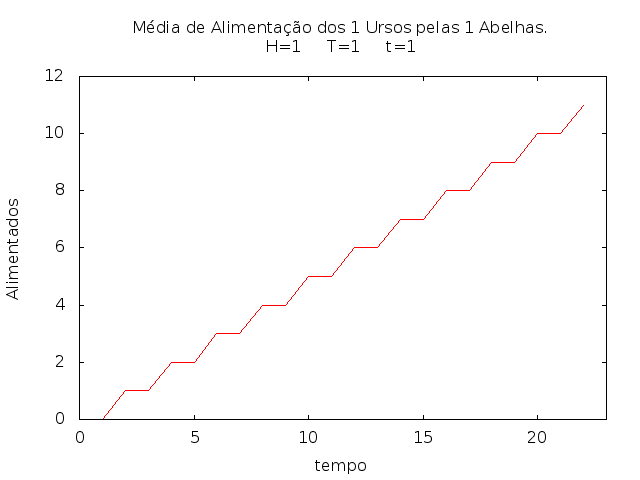
\includegraphics[width=0.7\paperwidth]{./graficos/ursos_1_1_1_1_1.png}
\label{Rotulo}
\end{figure}

\begin{figure}[!htb]
\centering
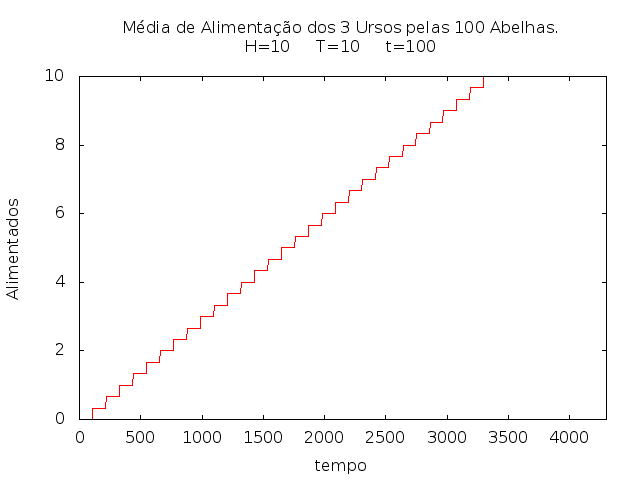
\includegraphics[width=0.7\paperwidth]{./graficos/ursos_100_3_10_100_10.png}
\label{Rotulo}
\end{figure}

\begin{figure}[!htb]
\centering
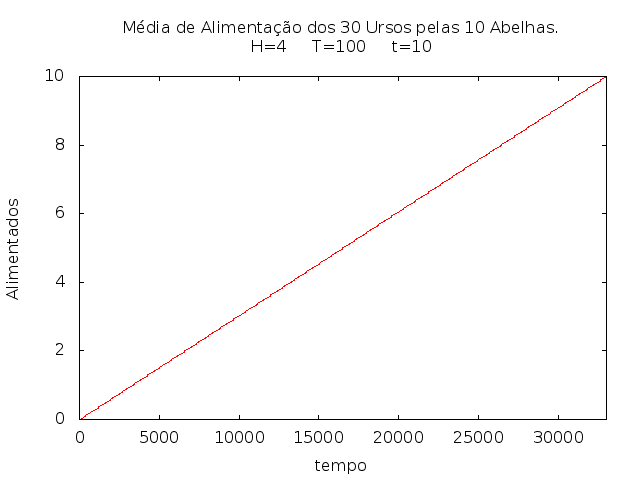
\includegraphics[width=0.7\paperwidth]{./graficos/ursos_10_30_4_10_100.png}
\label{Rotulo}
\end{figure}

\begin{figure}[!htb]
\centering
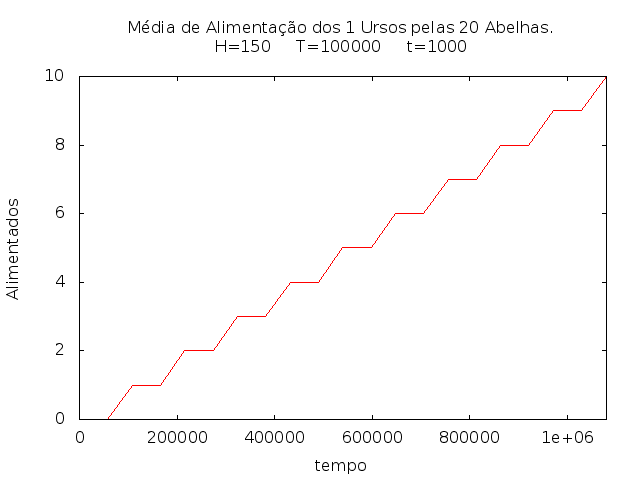
\includegraphics[width=0.7\paperwidth]{./graficos/ursos_20_1_150_1000_100000.png}
\label{Rotulo}
\end{figure}

\begin{figure}[!htb]
\centering
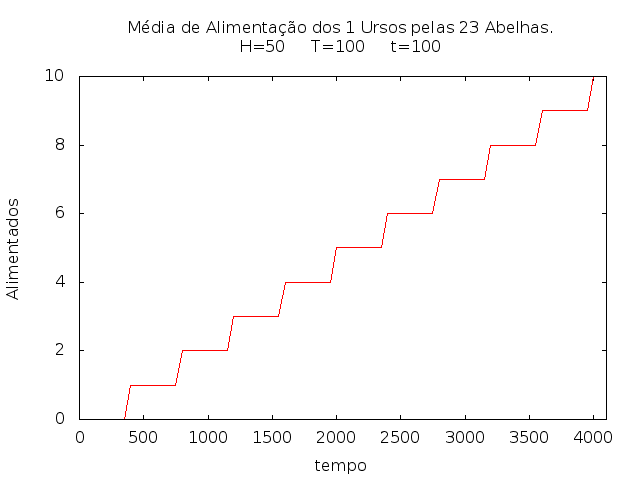
\includegraphics[width=0.7\paperwidth]{./graficos/ursos_23_1_50_100_100.png}
\label{Rotulo}
\end{figure}

\begin{figure}[!htb]
\centering
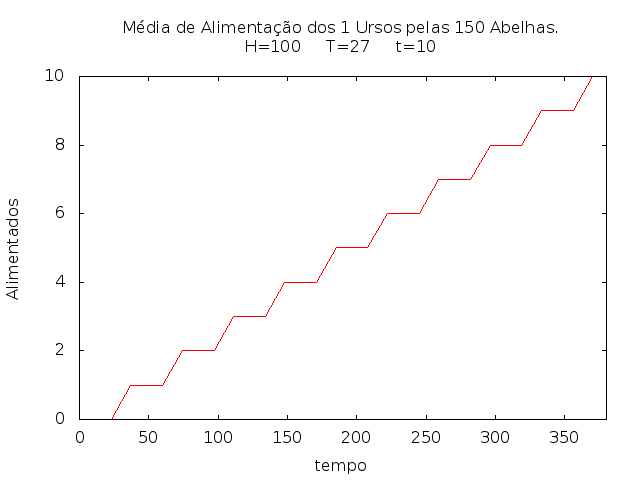
\includegraphics[width=0.7\paperwidth]{./graficos/ursos_150_1_100_10_27.png}
\label{Rotulo}
\end{figure}

\begin{figure}[!htb]
\centering
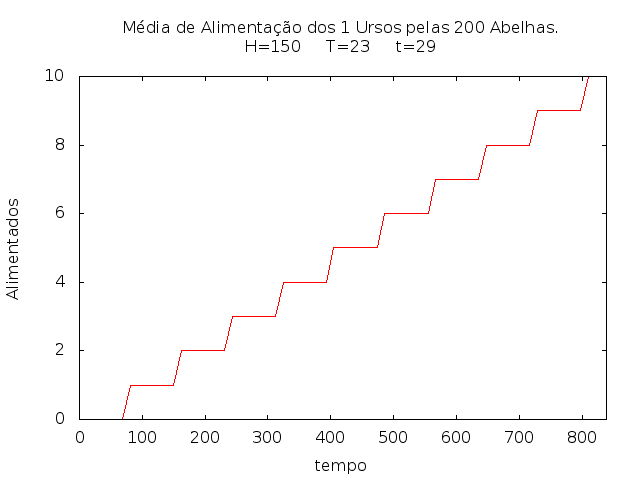
\includegraphics[width=0.7\paperwidth]{./graficos/ursos_200_1_150_29_23.png}
\label{Rotulo}
\end{figure}

\begin{figure}[!htb]
\centering
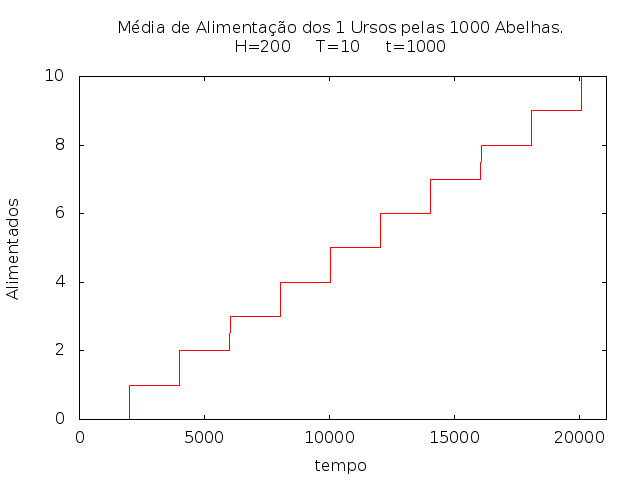
\includegraphics[width=0.7\paperwidth]{./graficos/ursos_1000_1_200_1000_10.png}
\label{Rotulo}
\end{figure}

\clearpage
\subsection{Abelhas:}

Este gráfico contém a média do número de vezes que cada abelha acordou um urso. Neste gráfico também é possível notar um formato de escada, já que as abelhas não produzem enquanto um urso se alimenta.

\begin{figure}[!htb]
\centering
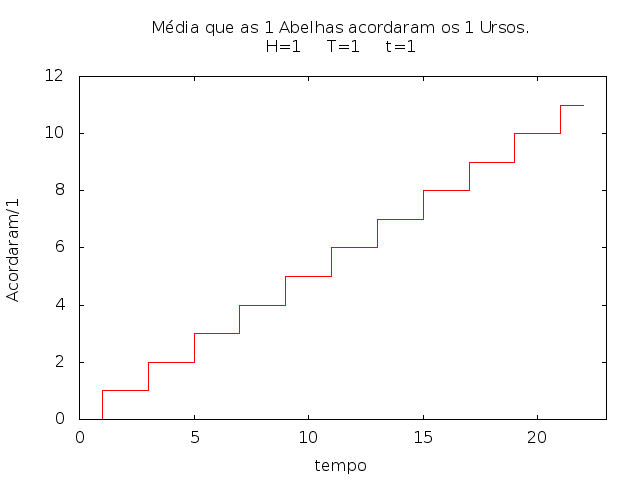
\includegraphics[width=0.7\paperwidth]{./graficos/abelhas_1_1_1_1_1.png}
\label{Rotulo}
\end{figure}


\begin{figure}[!htb]
\centering
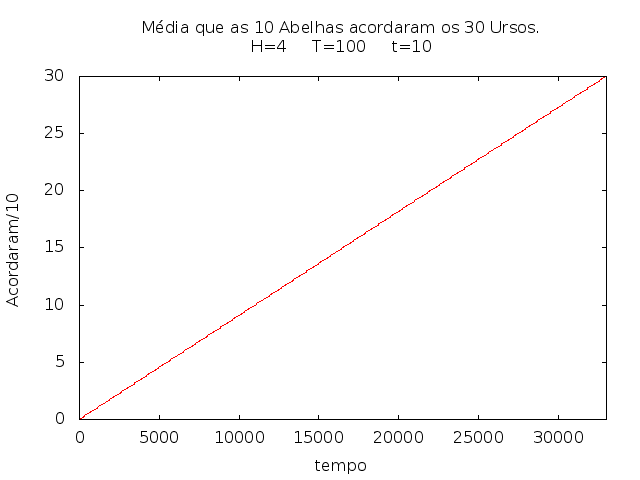
\includegraphics[width=0.7\paperwidth]{./graficos/abelhas_10_30_4_10_100.png}
\label{Rotulo}
\end{figure}

\begin{figure}[!htb]
\centering
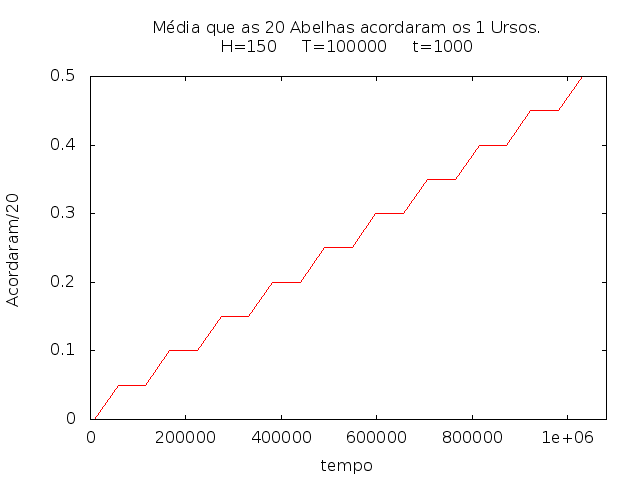
\includegraphics[width=0.7\paperwidth]{./graficos/abelhas_20_1_150_1000_100000.png}
\label{Rotulo}
\end{figure}

\begin{figure}[!htb]
\centering
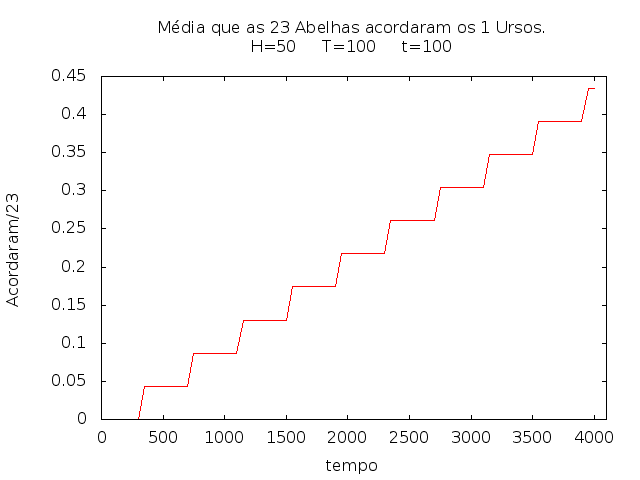
\includegraphics[width=0.7\paperwidth]{./graficos/abelhas_23_1_50_100_100.png}
\label{Rotulo}
\end{figure}

\begin{figure}[!htb]
\centering
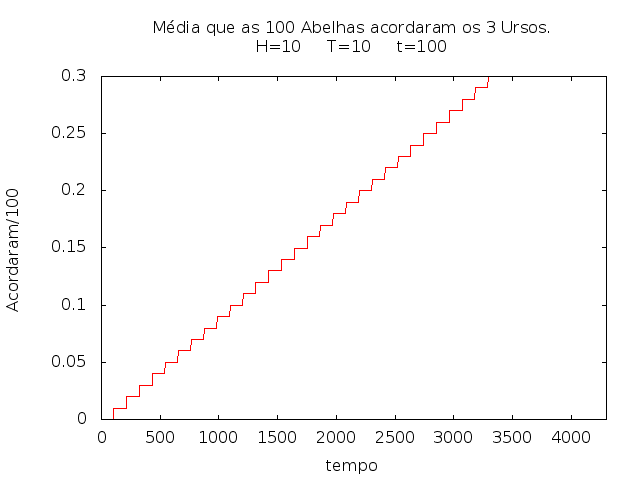
\includegraphics[width=0.7\paperwidth]{./graficos/abelhas_100_3_10_100_10.png}
\label{Rotulo}
\end{figure}

\begin{figure}[!htb]
\centering
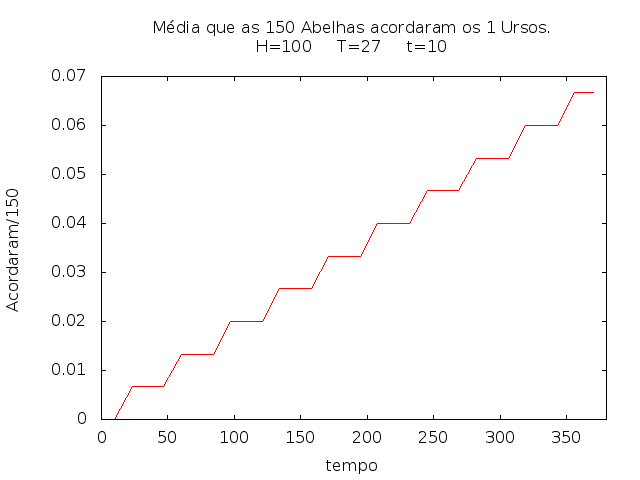
\includegraphics[width=0.7\paperwidth]{./graficos/abelhas_150_1_100_10_27.png}
\label{Rotulo}
\end{figure}

\begin{figure}[!htb]
\centering
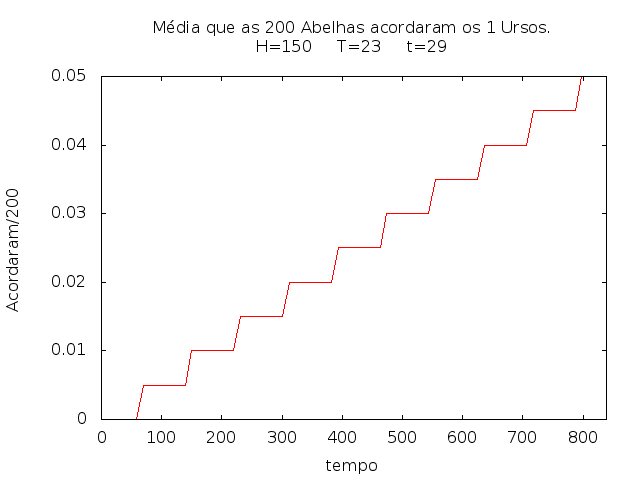
\includegraphics[width=0.7\paperwidth]{./graficos/abelhas_200_1_150_29_23.png}
\label{Rotulo}
\end{figure}

\begin{figure}[!htb]
\centering
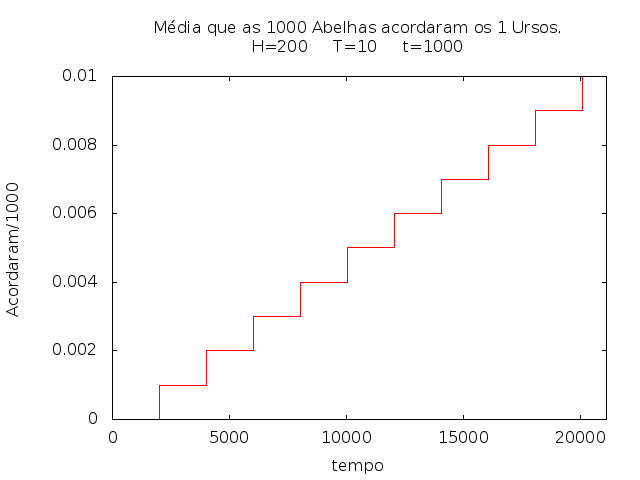
\includegraphics[width=0.7\paperwidth]{./graficos/abelhas_1000_1_200_1000_10.png}
\label{Rotulo}
\end{figure}

\clearpage
\subsection{Histograma:}

Também achamos interessante criar um gráfico que contabilize o acesso das abelhas ao pote. Portanto criamos um histograma com o número de acessos ao pote pelo id da abelha. As abelhas tiveram acesso muito bem distribuído ao pote mas não justo, fazendo com que algumas abelhas acessem mais o pote que outras.

\begin{figure}[!htb]
\centering
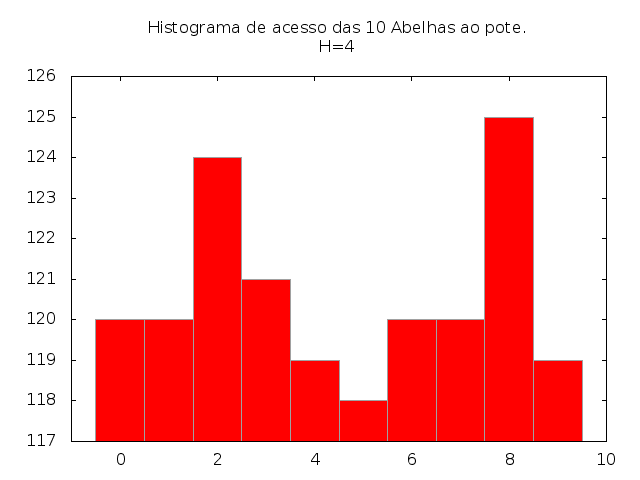
\includegraphics[width=0.7\paperwidth]{./graficos/histograma_10_30_4_10_100.png}
\label{Rotulo}
\end{figure}

\begin{figure}[!htb]
\centering
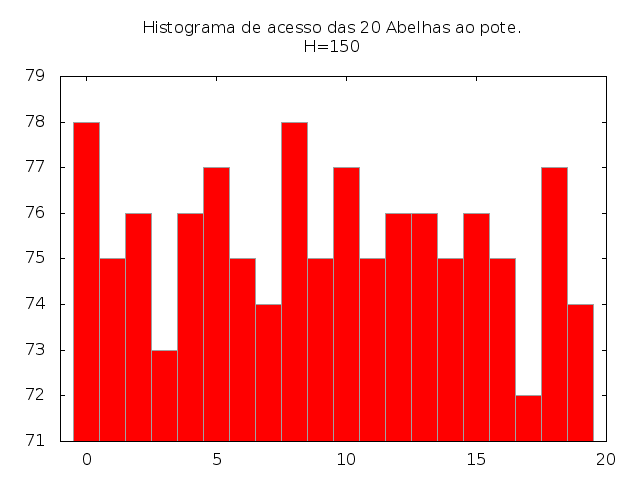
\includegraphics[width=0.7\paperwidth]{./graficos/histograma_20_1_150_1000_100000.png}
\label{Rotulo}
\end{figure}

\begin{figure}[!htb]
\centering
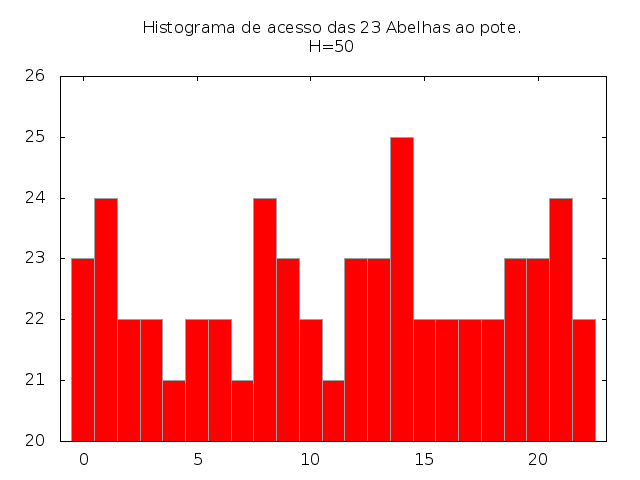
\includegraphics[width=0.7\paperwidth]{./graficos/histograma_23_1_50_100_100.png}
\label{Rotulo}
\end{figure}

\begin{figure}[!htb]
\centering
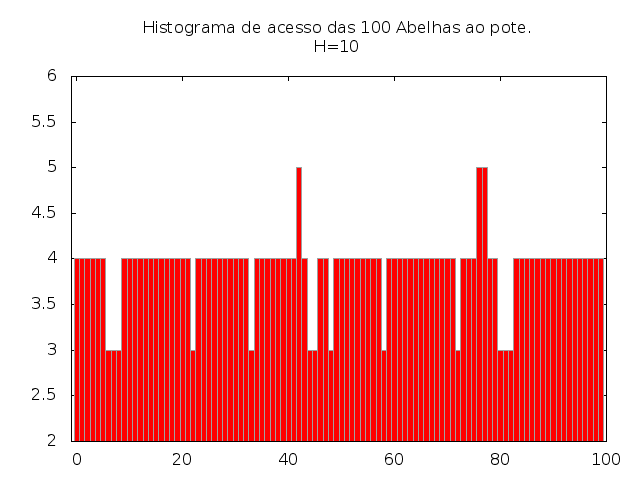
\includegraphics[width=0.7\paperwidth]{./graficos/histograma_100_3_10_100_10.png}
\label{Rotulo}
\end{figure}

\begin{figure}[!htb]
\centering
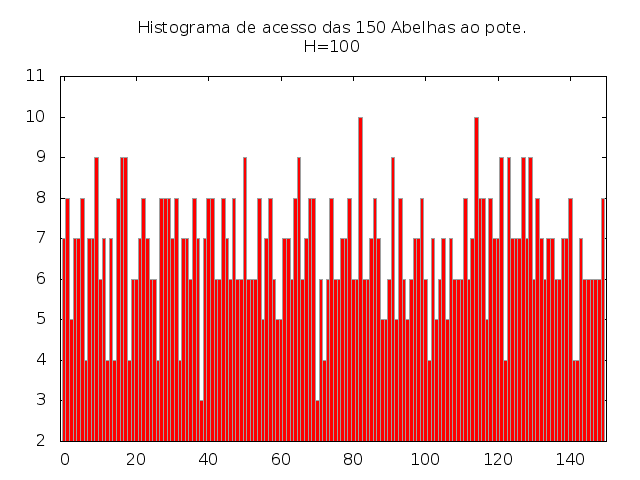
\includegraphics[width=0.7\paperwidth]{./graficos/histograma_150_1_100_10_27.png}
\label{Rotulo}
\end{figure}

\begin{figure}[!htb]
\centering
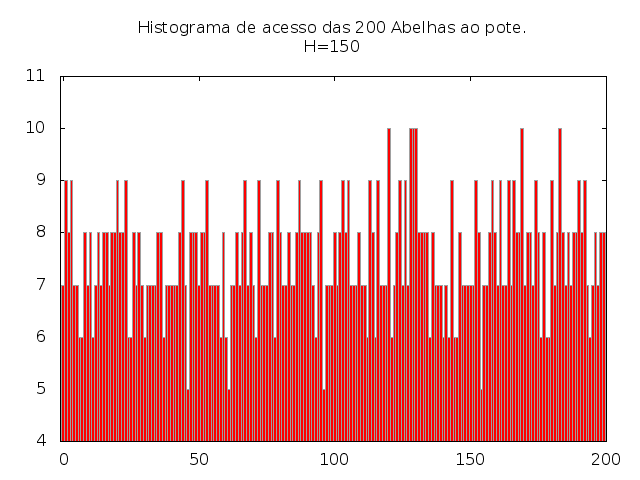
\includegraphics[width=0.7\paperwidth]{./graficos/histograma_200_1_150_29_23.png}
\label{Rotulo}
\end{figure}

\begin{figure}[!htb]
\centering
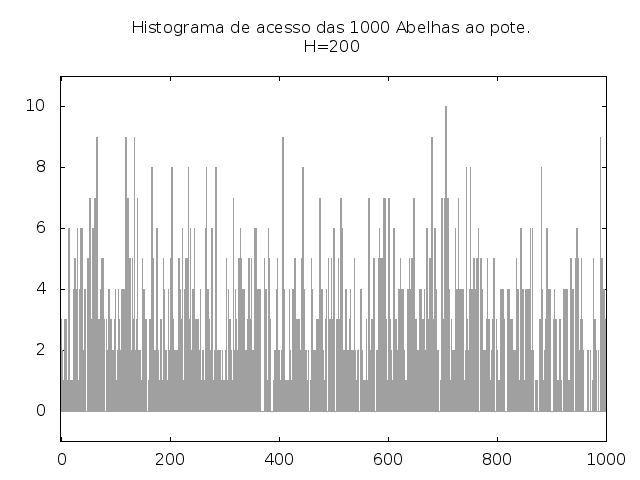
\includegraphics[width=0.7\paperwidth]{./graficos/histograma_1000_1_200_1000_10.png}
\label{Rotulo}
\end{figure}

\clearpage
\section{Conclusão}

Foi possível observar que o desenvolvimento de monitores para controle de acesso a recursos é algo bastante útil quando o problema tenha uma complexidade concorrete bastante elevada e a sessão crítica acabe sendo acessada em sequência. Neste caso é interessante criar uma classe que formalize de maneira mais adequada o problema. No entanto quando apenas poucas áreas de sessão crítica existem e elas tomam muito pouco tempo de processamento, então esta é uma solução pouco eficiente.

\end{document}
